\documentclass[11pt]{article}
\newcommand{\model}[1]{\texttt{#1}}

% Change "review" to "final" to generate the final (sometimes called camera-ready) version.
% Change to "preprint" to generate a non-anonymous version with page numbers.
\usepackage[review]{acl}

\usepackage{times}
\usepackage{latexsym}
\usepackage{colortbl}
\providecommand\UseTaggingSocket[1]{}
\usepackage[breakable]{tcolorbox}

\usepackage[T1]{fontenc}
\usepackage[utf8]{inputenc}
\usepackage{microtype}

\usepackage{inconsolata}
\usepackage{booktabs}
\usepackage{amsmath}
\usepackage{url}
\usepackage{graphicx}
\usepackage{tikz}
\usetikzlibrary{shapes.callouts, positioning, arrows.meta, calc, decorations.pathreplacing}
\setlength{\textfloatsep}{6pt plus 1pt minus 1pt}
\setlength{\floatsep}{6pt plus 1pt minus 1pt}
\setlength{\intextsep}{6pt plus 1pt minus 1pt}
\setlength{\dbltextfloatsep}{6pt plus 1pt minus 1pt}
\setlength{\dblfloatsep}{6pt plus 1pt minus 1pt}
\setlength{\abovecaptionskip}{3pt}
\setlength{\belowcaptionskip}{1pt}
\setlength{\abovedisplayskip}{4pt plus 1pt minus 1pt}
\setlength{\belowdisplayskip}{4pt plus 1pt minus 1pt}
\setlength{\abovedisplayshortskip}{2pt plus 1pt}
\setlength{\belowdisplayshortskip}{3pt plus 1pt minus 1pt}
\setlength{\parskip}{0pt plus 0.5pt}
\definecolor{tableheader}{gray}{0.85}
\definecolor{tablerow}{gray}{0.95}
\definecolor{figblue}{HTML}{3B82F6}
\definecolor{figred}{HTML}{EF4444}
\newcommand{\lightrule}{\arrayrulecolor{black!20}\midrule\arrayrulecolor{black}}
\setlength{\heavyrulewidth}{0.02em}
\setlength{\lightrulewidth}{0.02em}

\title{The Art of Saying No: BATNA-Aware Reward Design for LLM Strategic Negotiation}

\author{
  \textbf{Dhruv Bansal},
  \textbf{Bradley Breisch},
  \textbf{Rui Yin},
  \textbf{Wenhui Zhu},
  \textbf{Yaling Wang}
\\
  Arizona State University \\
  \small{
    \texttt{\{dbansa11, bbreisc1, ryin12, wzhu59, ylwang\}@asu.edu}
  }
}

\begin{document}
\maketitle
\raggedbottom

\begin{abstract}
Reinforcement learning enables the training of large language model (LLM) negotiation agents without human supervision. However, existing methods are often fragmented between disjoint task types and heavily rely on surplus rewards that treat the finalized agreement as superior to no deal. To address this, we ground our reward design in the bargaining theory of Best Alternative to a Negotiated Agreement (BATNA), positing that a rational agent should walk away rather than accept a contract below a critical quality threshold. We formalize this formulation as a parameterized utility floor and apply it selectively to multi-item scenarios where no task-given utility floor exists, while retaining surplus rewards for price bargaining settings. We train a single unified agent across four distinct price and multi-item benchmarks, evaluating its performance against both fixed and frontier opponents alongside a held-out dataset featuring a hybrid, multi-attribute structure. Our reward modeling achieves the highest average bargained ratio against both the fixed training opponent and a stronger frontier opponent, outperforming both surplus-based training and far larger frontier models while effectively eliminating the deal-closing bias on tasks where baseline incentives fail to distinguish fair compromises from poor agreements.
\end{abstract}

\section{Introduction}

Negotiation research has progressed from early neural models \citep{lewis2017deal, he2018decoupling} to large language model \citep[LLM;][]{minaee2024llmsurvey} benchmarks spanning price bargaining and multi-item allocation \citep{xia2024measuring, kwon2024llmseffectivenegotiators, bianchi2024negotiationarena, noh2024personalities, chatterjee2024agreemate, hua2024gametheoretic}, revealing that even frontier models routinely accept negative-utility deals. Reinforcement learning has been used to address this gap \citep{liu2026instructing, bergemann2026bilateral, vendrell2026gametalk, zeng2025repo, long2025evoemo, oh2026merit}, but existing methods typically train on a single task type and rely on surplus rewards that treat any closed \emph{multi-item} deal as positive (\S\ref{sec:reward}). The Best Alternative to a Negotiated Agreement (BATNA) \citep{fisher1981gettingtoyes}, the principle that rational negotiators should prefer walking away to accepting deals worse than their outside option, has not been incorporated into reward design.

\begin{figure}[t]
\centering
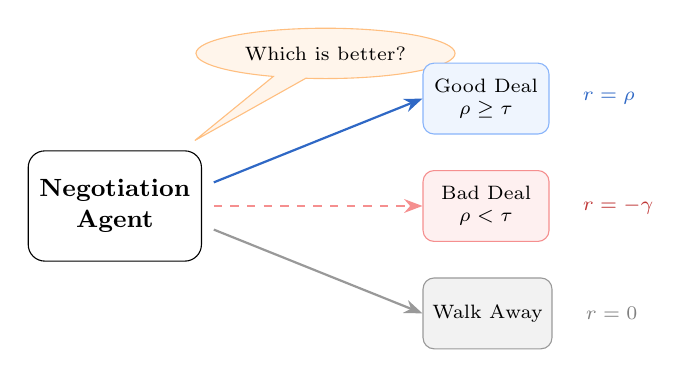
\begin{tikzpicture}[
  >=Stealth,
  agent/.style={
    rectangle, rounded corners=6pt, draw=black, fill=white,
    minimum width=2.2cm, minimum height=1.4cm, align=center,
    font=\small\bfseries
  },
  thought/.style={
    ellipse callout, draw=orange!50, fill=orange!8,
    callout relative pointer={(#1)},
    font=\scriptsize, align=center, inner sep=4pt
  },
  deal/.style={
    rectangle, rounded corners=4pt, draw=figblue!60, fill=figblue!8,
    minimum width=1.6cm, minimum height=0.9cm, align=center,
    font=\scriptsize
  },
  bad/.style={
    rectangle, rounded corners=4pt, draw=figred!60, fill=figred!8,
    minimum width=1.6cm, minimum height=0.9cm, align=center,
    font=\scriptsize
  },
  walk/.style={
    rectangle, rounded corners=4pt, draw=black!40, fill=gray!10,
    minimum width=1.6cm, minimum height=0.9cm, align=center,
    font=\scriptsize
  },
  reward/.style={font=\scriptsize\bfseries},
]

% Agent
\node[agent] (agent) {Negotiation\\Agent};

% Thought bubble
\node[thought={(-1.2cm, -0.8cm)}, above right=1.0cm and 0.4cm of agent]
  (bubble) {Which is better?};

% Good deal
\node[deal, above right=0.2cm and 2.8cm of agent] (good)
  {Good Deal\\$\rho \geq \tau$};
\node[reward, right=0.3cm of good, figblue!80!black] {$r = \rho$};

% Bad deal
\node[bad, right=2.8cm of agent] (bad)
  {Bad Deal\\$\rho < \tau$};
\node[reward, right=0.3cm of bad, figred!80!black] {$r = -\gamma$};

% Walk away
\node[walk, below right=0.2cm and 2.8cm of agent] (walk)
  {Walk Away};
\node[reward, right=0.3cm of walk, black!50] {$r = 0$};

% Arrows from agent
\draw[->, thick, figblue!80!black]
  (agent.east) ++(0.15,0.3) -- (good.west);
\draw[->, thick, figred!60, dashed]
  (agent.east) ++(0.15,0) -- (bad.west);
\draw[->, thick, black!40]
  (agent.east) ++(0.15,-0.3) -- (walk.west);

\end{tikzpicture}
\caption{Training the agent to incorporate the BATNA principle by enforcing an abstract quality threshold $\tau$ rather than accepting sub-optimal deals.}
\label{fig:batna_hero}
\end{figure}

Surplus rewards are reasonable for single-item price bargaining, where the seller's reservation price floors deal quality, but fail in multi-item settings where no such floor exists. \citet{bergemann2026bilateral} diagnose this directly: surplus-only training produces a deal-closing bias where agents optimize for closure rather than quality. Meanwhile, \citet{liu2026instructing} show that verifiable rewards alone produce sophisticated strategic behavior (including aggressive anchoring and multi-turn persuasion) on a single price dataset, and \citet{chawla2023selfish} find that self-interested agents outperform fairness-oriented ones. The missing piece is a negative signal for low-quality multi-item deals, but it must be selective: applying a threshold uniformly would penalize thin-margin price agreements.

We provide this selective signal and train a single agent across four benchmarks spanning both task types, evaluating on a held-out fifth dataset. Our contributions are threefold: (1) we introduce a BATNA-aware threshold reward that teaches negotiation agents to prefer walking away over accepting low-quality agreements; (2) we show that reward design in negotiation should be selective, applying threshold-based penalties only to task settings lacking natural utility floors; and (3) we train a unified negotiation agent across heterogeneous benchmarks and demonstrate improved deal quality, reduced deal-closing bias, and transfer to unseen negotiation structures compared to both surplus-based training and frontier LLM baselines.\footnote{All training and evaluation code, configuration files, and data splits will be released upon publication.} % TODO(resubmission): replace footnote with anonymized repository URL.

\section{Methodology}

We model negotiation as a single-agent Markov Decision Process (MDP) in which only the learner's policy is optimized; while the opponent is a frozen language model forming part of the environment. Following \citet{he2018decoupling}, each turn consists of a private thought hidden from the opponent, a visible utterance, and a formal action: \textbf{Submit Deal}, \textbf{Accept Deal}, \textbf{Reject Deal}, or \textbf{Walk Away}. A \textbf{Submit Deal} corresponds to a price proposal in price scenarios and an item allocation in multi-issue scenarios. In price tasks, the learner is always the buyer and the opponent the seller; in CaSiNo and DnD, roles are symmetric and randomly assigned; in JI, the learner is always the job applicant. A regulation mechanism intercepts opponent actions that would yield negative utility, replacing them with rejections to prevent exploitation of irrational concessions; this control applies only to the frozen opponent, and the learner never accesses its counterpart's constraints. Episodes end on agreement, walk-away, $T{=}6$ rounds per agent, format violations (training), or reject loops (evaluation).

Modeling the opponent as a frozen copy of the base model rather than a co-adapting self-play agent isolates the effect of reward design: a stationary opponent ensures that differences between surplus and threshold training arise from the reward function alone, not from environmental non-stationarity.

Regulation creates an asymmetry. In price scenarios, it keeps the price $P$ at or above the seller's cost $\mathcal{C}$, and the task's reservation values give a quality reference where overpaying is penalized through $\rho < 0$. In multi-item scenarios no such reference exists, and a cooperative opponent may accept lopsided splits that yield the learner minimal utility. This motivates the selective reward design in \S\ref{sec:reward}.

\begin{figure}[t]
\centering
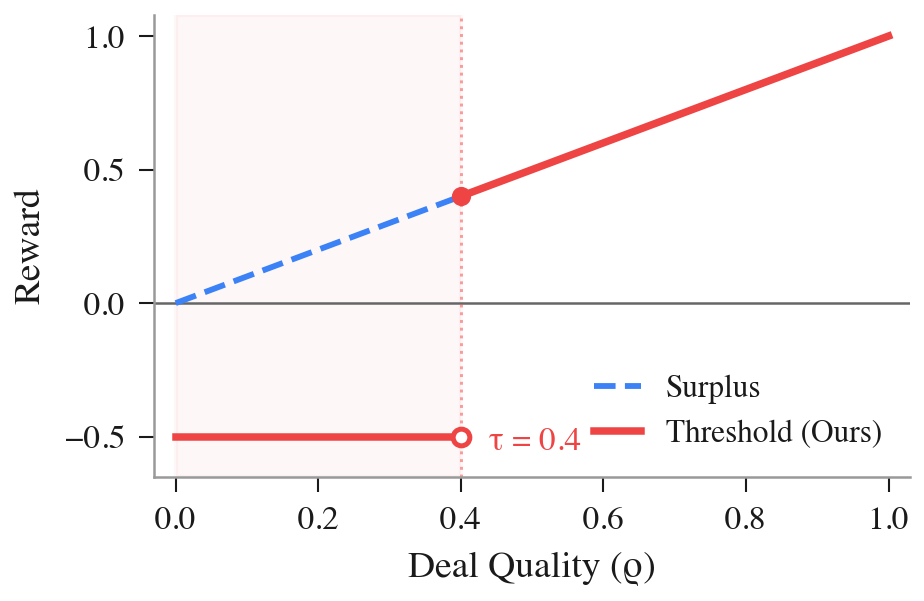
\includegraphics[width=\columnwidth]{figures/reward_design.png}
\caption{Surplus vs.\ threshold reward for multi-item scenarios; threshold rewards discourage poor deals.}
\label{fig:reward_design}
\end{figure}

\subsection{Reward Design}
\label{sec:reward}

The reward is terminal and verifiable, computed solely from deal terms and private constraints at episode end, requiring no learned reward model or human annotation. We measure deal quality by the \textit{bargained ratio} $\rho$, the fraction of maximum surplus captured by the learner: $\rho_{\textit{price}} = (\mathcal{B} - P) / |\mathcal{B} - \mathcal{C}|$ for a buyer with budget $\mathcal{B}$ negotiating price $P$ against a seller with cost $\mathcal{C}$, and $\rho_{\textit{multi}} = u(x) / u(x^*)$ for multi-item allocation with achieved utility $u(x)$ and maximum $u(x^*)$. Normalizing by the maximum possible surplus makes deal quality comparable across scenarios with different value scales, enabling a single reward function across heterogeneous benchmarks.

\paragraph{Surplus reward.} Following \citet{liu2026instructing}, any closed deal receives $\rho$ as reward and all other outcomes receive zero. In price bargaining this can penalize bad deals, since task-given reservation values allow $\rho < 0$ when the buyer overpays. In multi-item allocation, however, item values are non-negative, so $\rho \in [0,1]$ for \textit{every} feasible allocation: a utility floor cannot arise from the task and must be imposed by the reward designer. Surplus rewards therefore conflate two distinct signals in multi-item settings: \textit{whether} a deal was reached and \textit{whether} it was good. A policy that consistently closes low-quality deals therefore gains positive advantage over policies that walk away, reinforcing deal-closing even when disagreement would be the rational outcome.

\paragraph{Threshold Reward Modeling.} To operationalize the BATNA principle, we introduce a parameterized quality threshold $\tau \in [0, 1]$ for multi-item scenarios (Figure~\ref{fig:reward_design}). Completed deals with normalized surplus $\rho$ satisfying $\rho \geq \tau$ receive reward $\rho$, while deals below $\tau$ receive a penalty $-\gamma$, making walk-away outcomes preferable. Formally, the reward $R(x)$ for a contract $x$ is: $R(x) = 
\rho$ if $\rho \geq \tau$, and $R(x) = 
-\gamma$ otherwise, where no-deal outcomes receive $0$ and format violations receive $-\psi$. This asymmetry is deliberate. In price bargaining, the task's reservation values already give a quality reference, so a strict threshold would penalize legitimately thin-margin agreements. In multi-item settings, no such reference exists, making the threshold necessary to establish a utility floor. The abstract parameter balances rewarding compromises against filtering lopsided agreements without tying the formulation to a specific task distribution while price settings retain the original surplus reward.

\begin{table}[t]
\centering
\scriptsize
\setlength{\tabcolsep}{3pt}
\renewcommand{\arraystretch}{1.15}
\begin{tabular}{l c c c c c}
\toprule
\rowcolor{tableheader}
\textbf{Model} & \textbf{AHP} & \textbf{CA} & \textbf{CRA} & \textbf{DnD} & \textbf{JI} \\
\midrule
\rowcolor{tablerow}
Threshold (Ours) & \textbf{.80} (79) & \textbf{.58} (76) & \textbf{.65} (87) & \textbf{.70} (78) & .70 (83) \\
Surplus  & \underline{.64} (75)          & \textbf{.58} (78) & \underline{.61} (89) & .55 (\textbf{90}) & .63 (\underline{91}) \\
\lightrule
\rowcolor{tablerow}
Qwen3-30B        & $-.05$ (71)       & .52 (61)          & .01 (63)       & .67 (59)          & .71 (57)          \\
Qwen3-30B-T      & .17 (76)          & .49 (70)          & .02 (69)          & .55 (70)          & \textbf{.79} (46) \\
\rowcolor{tablerow}
Qwen3-235B       & .34 (80)          & .55 (51)          & .14 (84)          & .63 (83)          & .74 (75)          \\
Qwen3-235B-T     & .32 (90)          & .50 (60)          & .19 (85)          & .55 (71)          & .74 (72)          \\
\rowcolor{tablerow}
Qwen3.6-35B-A3B  & .46 (81)          & .50 (33)          & .24 (62)          & .60 (47)          & .63 (33)          \\
GPT-5.4          & .52 (\underline{92}) & .52 (63) & .27 (89) & \underline{.69} (\underline{90}) & .73 (78) \\
\rowcolor{tablerow}
GPT-5.4-mini     & .47 (72)          & .47 (57)          & .12 (81)          & .65 (83)          & .71 (85)          \\
DeepSeek-V3.1    & .41 (\textbf{94}) & .49 (69)          & .18 (89)          & .63 (85)          & \underline{.77} (82) \\
\rowcolor{tablerow}
Kimi-K2-T        & .42 (\textbf{94}) & .45 (78)          & .19 (\underline{91}) & .64 (87)       & .73 (88)          \\
Llama-4-Maverick      & .07 (85)      & .51 (76)          & $-.08$ (72)       & .57 (89)          & .76 (\textbf{94}) \\
\bottomrule
\end{tabular}

\caption{Bargained ratio and deal rate (\%, in parentheses) against \model{Qwen3-30B-A3B}. T = Thinking variant.}
\label{tab:results-qwen}
\end{table}

\section{Experimental Results}

\begin{figure}[t]
\centering
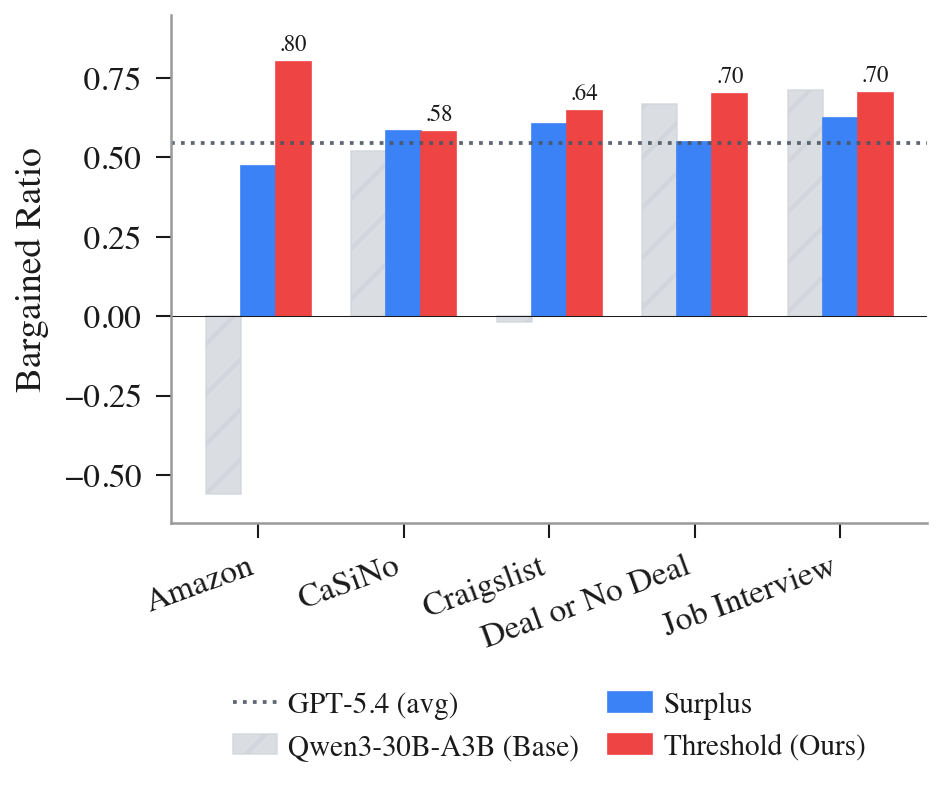
\includegraphics[width=\columnwidth]{figures/bar_results.png}
\caption{Bargained ratio across five benchmarks. Job Interview is held out from training.}
\label{fig:bar_results}
\end{figure}

We fine-tune \model{Qwen3-30B-A3B-Instruct} \citep{qwen2025qwen3} with Group Relative Policy Optimization \citep{shao2024deepseekmath} and LoRA against a frozen copy of the base model as opponent (full setup in Appendix~\ref{app:training}). Training draws uniformly from four datasets: AmazonHistoryPrice (AHP; \citealp{xia2024measuring}) and CraigslistBargains (CRA; \citealp{he2018decoupling}) for price bargaining, CaSiNo (CA; \citealp{chawla2021casino}) and Deal or No Deal (DnD; \citealp{lewis2017deal}) for multi-item allocation. Each step generates 512 rollouts without a KL penalty; reward curves plateau well before step~80 (Figure~\ref{fig:reward_curves}). We evaluate on held-out test splits of the four training datasets plus a held-out Job Interview dataset (JI; \citealp{yamaguchi2021dialogue}) combining salary negotiation with multi-attribute allocation, using 100 scenarios per dataset (temperature $0.7$, $p{=}0.9$). We clip the bargained ratio to $[-1,1]$ when reporting so a few degenerate thin-margin price episodes cannot dominate the mean.

Table~\ref{tab:results-qwen} reports bargained ratio and deal rate against the frozen training opponent. The threshold agent achieves the highest average bargained ratio at $0.69$, outperforming surplus at $0.60$, \model{GPT-5.4} at $0.54$, and \model{DeepSeek-V3.1} at $0.50$ (Figure~\ref{fig:bar_results}). The early reward gap in Figure~\ref{fig:reward_curves} reflects the penalty on low-quality deals, which closes as the agent learns to avoid them. Untrained models struggle most on price bargaining: on AHP and CRA, base models score near zero or negative because they concede to the seller's anchor. On average, threshold scores $0.72$ bargained ratio on price tasks versus $0.62$ for surplus, and $0.64$ on multi-item tasks versus $0.57$.

\begin{figure}[t]
\centering
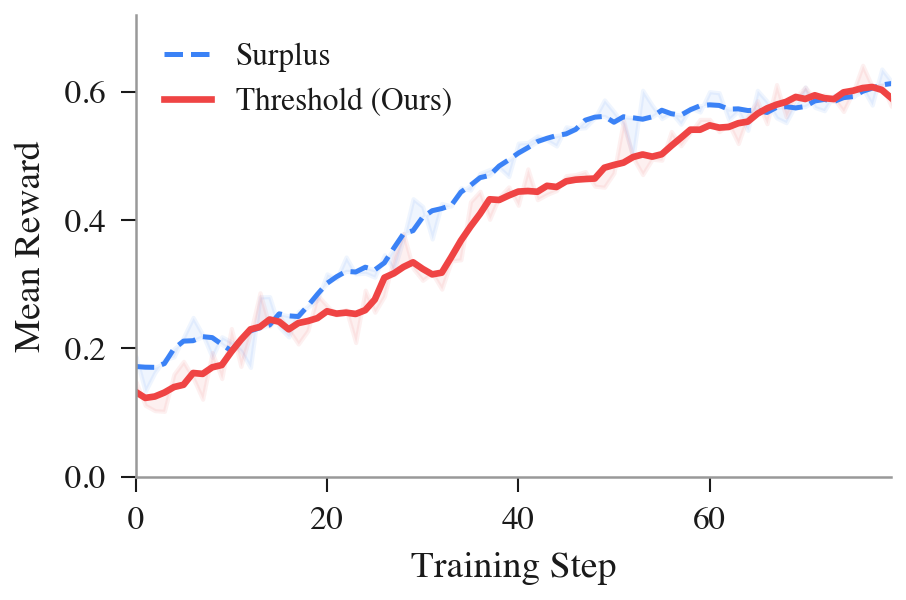
\includegraphics[width=\columnwidth]{figures/reward_curves.png}
\caption{Mean reward during training. Lines show the 5-step moving average; shaded bands span the raw per-step reward around it, reflecting step-to-step training noise rather than a confidence interval.}
\label{fig:reward_curves}
\end{figure}

\paragraph{Quality over closure.}
The sharpest contrast between reward designs appears on multi-item tasks. On DnD, the surplus agent closes $90\%$ of deals but at $0.55$ bargained ratio; the threshold agent closes $78\%$ at $0.70$ (Table~\ref{tab:results-qwen}). Surplus training produces the deal-closing bias \citet{bergemann2026bilateral} diagnose, accepting lopsided splits rather than walking away; the threshold reward inverts this by making bad deals worse than no deal. The surviving deals are also more jointly efficient: DnD Pareto efficiency rises from $0.29$ (surplus) to $0.50$ (threshold), since lopsided splits sit far from the efficient frontier (Table~\ref{tab:fbr_pareto_vs_qwen}).

\begin{table}[!t]
\centering
\scriptsize
\setlength{\tabcolsep}{3pt}
\renewcommand{\arraystretch}{1.15}
\begin{tabular}{l cc cc}
\toprule
\rowcolor{tableheader}
& \multicolumn{2}{c}{\textbf{Pareto} ($\uparrow$)} & \multicolumn{2}{c}{\textbf{1st-Bid} ($\downarrow$)} \\
\rowcolor{tableheader}
\textbf{Model} & \textbf{CA} & \textbf{DnD} & \textbf{AHP} & \textbf{CRA} \\
\midrule
\rowcolor{tablerow}
Threshold (Ours) & .58          & .50          & \textbf{.36} & \textbf{.40} \\
Surplus   & .49          & .29          & \underline{.59} & \underline{.56} \\
\lightrule
\rowcolor{tablerow}
Qwen3-30B        & .44          & .31          & .95          & .92 \\
Qwen3-30B-T      & .51          & \underline{.51} & .92       & .91 \\
\rowcolor{tablerow}
Qwen3-235B       & .41          & .41          & .81          & .84 \\
Qwen3-235B-T     & .52          & .42          & .81          & .85 \\
\rowcolor{tablerow}
Qwen3.6-35B-A3B  & \underline{.61} & .49          & .78          & .84 \\
GPT-5.4          & .38          & \textbf{.60} & .72          & .78 \\
\rowcolor{tablerow}
GPT-5.4-mini     & .44          & .50          & .75          & .83 \\
DeepSeek-V3.1    & .39          & .42          & .75          & .82 \\
\rowcolor{tablerow}
Kimi-K2-T        & \textbf{.64} & \underline{.52} & .82       & .85 \\
Llama-4-Maverick      & .47          & .42          & .91          & .95 \\
\bottomrule
\end{tabular}
\caption{Pareto efficiency (multi-item, $\uparrow$) and first-bid ratio (price, $\downarrow$) vs.\ \model{Qwen3-30B-A3B}. T = Thinking.}
\label{tab:fbr_pareto_vs_qwen}
\end{table}

\begin{figure}[t]
\centering
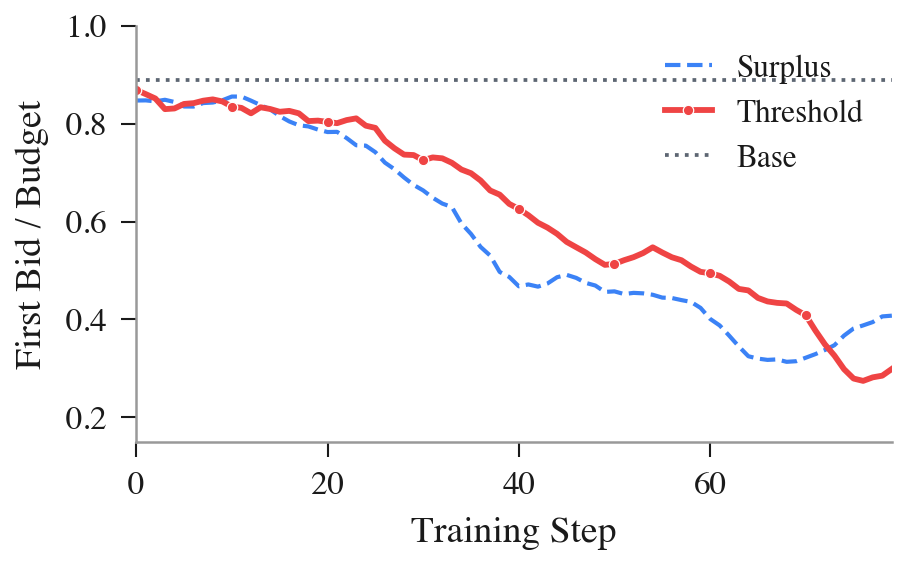
\includegraphics[width=\columnwidth]{figures/first_bid_ratio.png}
\caption{First-bid ratio (opening offer\,/\,budget) over training. The threshold agent reaches ${\approx}\,0.30$ while surplus plateaus at ${\approx}\,0.45$. Base model starts at ${\approx}\,0.89$.}
\label{fig:first_bid}
\end{figure}

\paragraph{Aggressive anchoring without deadlock.}
First-bid ratio, defined for price scenarios where the opening offer is a scalar, measures how aggressively the buyer anchors below budget \citep{galinsky2001firstoffers, xia2024measuring}. The threshold agent anchors far more aggressively than surplus or the base model: its first-bid ratio falls to ${\approx}\,0.30$ of budget over training (Figure~\ref{fig:first_bid}) and averages $0.36$/$0.40$ on AHP/CRA at evaluation, versus $0.59$/$0.56$ for surplus and $0.95$/$0.92$ for the base model (Table~\ref{tab:fbr_pareto_vs_qwen}), despite the threshold penalty applying only to multi-item deals. One might hypothesize that walk-away tolerance from multi-item training transfers to price as deeper anchoring; a controlled ablation rejects this (Appendix~\ref{app:transfer}): training on multi-item tasks alone yields no positive transfer to price, so the price gains stem from the direct price-task surplus reward rather than cross-task transfer. This signal drives the largest single-dataset gain: on AHP, bargained ratio recovers from $-0.05$ (base) to $0.80$.

\begin{figure}[t]
\centering
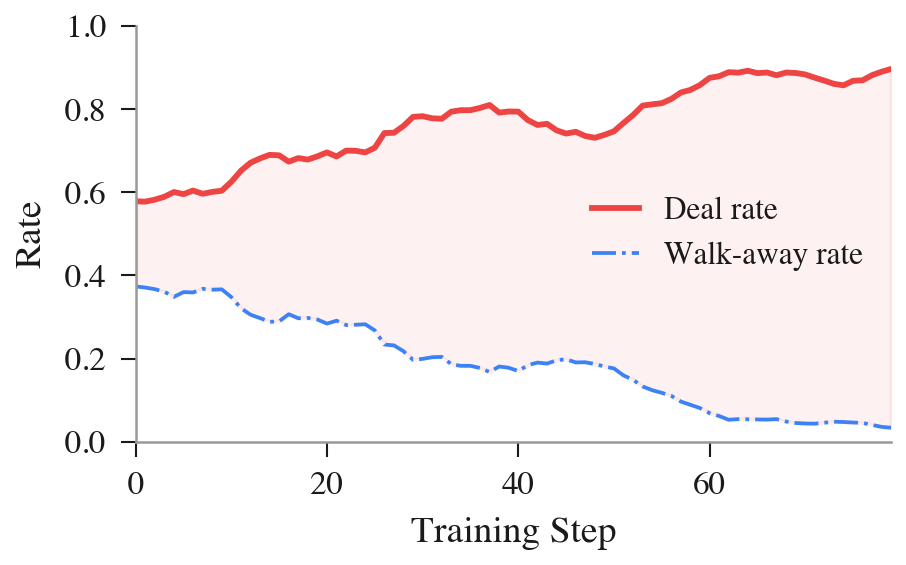
\includegraphics[width=\columnwidth]{figures/deal_walk_rate.png}
\caption{Deal and walk-away rates for the threshold agent. Deal rate increases monotonically with no deadlock phase.}
\label{fig:deal_walk}
\end{figure}

\paragraph{Cross-task transfer.}
Neither reward sees JI during training, yet the threshold agent reaches $0.70$ bargained ratio, comparable to frontier models $8$--$200{\times}$ larger (mostly $0.71$--$0.79$) and well above surplus ($0.63$). Quality discrimination learned on price and multi-item tasks thus generalizes to JI's hybrid structure without explicit exposure.

\paragraph{Selective deal-making.}
Figure~\ref{fig:deal_walk} shows selectivity and quality co-evolving: the agent initially walks away from sub-$\tau$ deals, but as it learns to negotiate better deals walk-away rates fall until deal rates approach surplus while bargained ratio stays higher. Unlike \citet{liu2026instructing}, who observe a deadlock phase under surplus training on a single price dataset, our agent bypasses this across the mixed tasks.

\section{Discussion}

Our fixed threshold is the simplest operationalization of the walk-away principle; a real outside option is context-dependent and shaped during negotiation \citep{fisher1981gettingtoyes, raiffa1982art}. Two extensions could add context sensitivity while preserving verifiability: a dynamic threshold conditioned on item configurations or opponent behavior, and an opponent-aware threshold informed by the Nash bargaining solution \citep{nash1950bargaining}. Extending the framework to evolving outside options and multi-deal relationships \citep{zeng2025repo} will likely require population-based or self-play training \citep{liu2025spiral}. More broadly, this asymmetry (structural quality floors in price bargaining, none in multi-item allocation) suggests reward design should be \textit{selective}, not universal.


\section*{Limitations}

Existing negotiation benchmarks in the NLP and financial AI communities evaluate agents on single-episode, complete-information settings, ignoring the sequential and information-asymmetric structure of real procurement and contract negotiation. This gap means that no current evaluation, including ours, tests whether learned strategies transfer to multi-round settings where each deal reshapes the next round's outside options. Separately, the regulation mechanism that prevents the opponent from accepting irrational deals assumes access to private constraints, an assumption shared by all controlled negotiation setups but absent in deployment; the trained policy itself, however, requires no access to its counterpart's constraints at inference time. Constructing multi-round, partial-information negotiation corpora and evaluating reward design under those conditions remains an open direction.

\section*{Acknowledgments}
AI coding assistants were used during codebase development and paper writing; all outputs were reviewed and validated by the authors.

\bibliography{references}
\clearpage

\appendix

\section{Training Details}
\label{app:training}

Both agents are fine-tuned from \model{Qwen3-30B-A3B-Instruct-2507} (30.5B total parameters, 3.3B activated per token) using Group Relative Policy Optimization \citep{shao2024deepseekmath} with LoRA. The two training runs differ only in the reward function: the threshold run penalizes multi-item deals with bargained ratio below $\tau = 0.4$ with penalty $\gamma{=}0.5$, while the surplus run rewards any closed deal proportionally to surplus captured. Format violations receive $-\psi$ with $\psi{=}1.0$ in both runs. All deal rewards are clipped to $[-1, 1]$ to bound gradient magnitude. Training and evaluation were conducted on the Tinker platform \citep{tinker2025}, a cloud-based RL fine-tuning API that handles distributed sampling and gradient computation. The total compute cost for both training runs and all evaluations was approximately \$250 USD. Table~\ref{tab:hyperparams} lists the shared hyperparameters.

\paragraph{Train/test splits.}
Training and evaluation draw from disjoint scenario pools. CaSiNo uses its standard split (906 training / 124 evaluation scenarios), retaining every row. DnD also uses its standard split (5{,}048 / 526 unique scenarios), with the two participant records for each negotiation combined into one scenario. CraigslistBargains uses its standard split, retaining 4{,}020 / 637 dialogues that contain a buyer knowledge base and a positive bargaining interval (the buyer target exceeds the seller cost, defined as 50\% of listing price). AmazonHistoryPrice provides no canonical split, so we create a category-stratified 80/20 product-level split (743 / 187 products); we retain 422 / 93 scenarios whose list, current, and historical-low prices are parseable and whose current price exceeds the historical low. Job Interview is excluded from training and serves as the held-out transfer benchmark, retaining 295 completed scenarios that contain both roles and an accepted solution. Evaluation samples scenarios exclusively from the held-out pools.

\begin{table}[ht]
\centering
\scriptsize
\renewcommand{\arraystretch}{1.15}
\begin{tabular}{ll}
\toprule
\rowcolor{tableheader}
\textbf{Hyperparameter} & \textbf{Value} \\
\midrule
\rowcolor{tablerow}
Base model & Qwen3-30B-A3B-Instruct \\
LoRA rank & 32 \\
\rowcolor{tablerow}
Learning rate & $3 \times 10^{-5}$ \\
Batch size & 64 scenarios/step \\
\rowcolor{tablerow}
Group size (GRPO) & 8 \\
Max negotiation rounds & 6 \\
\rowcolor{tablerow}
Max generation tokens & 512 \\
Train temperature & 1.0 (learner), 0.7 (opp.) \\
\rowcolor{tablerow}
Eval temperature & 0.7 (both), $p{=}0.9$ \\
KL penalty & 0.0 \\
Training steps & 80 \\
\rowcolor{tablerow}
Datasets & CA, DnD, AHP, CRA (25\% each) \\
\bottomrule
\end{tabular}
\caption{Training hyperparameters shared across both reward variants.}
\label{tab:hyperparams}
\end{table}

\section{Evaluation Metrics}
\label{app:metrics}

Beyond the bargained ratio $\rho$ defined in the main text, the analysis uses two auxiliary metrics, reported in Tables~\ref{tab:fbr_pareto_vs_qwen} and~\ref{tab:fbr_pareto_vs_gpt}.

\paragraph{First-bid ratio.} Defined for price scenarios, where the opening offer is a scalar, this measures how aggressively the buyer anchors below its budget. Let $P_1$ be the price in the learner's first \texttt{[SUBMIT\_DEAL]} action and $\mathcal{B}$ its private budget. Then
\begin{equation}
\text{first-bid ratio} = \frac{P_1}{\mathcal{B}},
\label{eq:first_bid}
\end{equation}
averaged over price episodes that contain an opening offer. Lower values indicate more aggressive anchoring; a buyer that opens at its full budget scores $1$.

\paragraph{Pareto efficiency.} Defined for multi-item allocation on closed deals. A deal assigns the learner an allocation $x$ and the opponent the complement $\bar{x}$, where $x$ and $\bar{x}$ partition the fixed item pool. Writing $u_L$ and $u_O$ for the learner's and opponent's private utilities and $\mathcal{X}$ for the set of all feasible integer allocations of the pool, the deal $x$ is Pareto efficient if no other feasible allocation makes one party better off without making the other worse off:
\begin{equation}
\neg\,\exists\, x' \in \mathcal{X}:\ u_L(x') \ge u_L(x)\ \wedge\ u_O(\bar{x}') \ge u_O(\bar{x}),
\label{eq:pareto}
\end{equation}
with at least one inequality strict. We report the Pareto efficiency \emph{rate}: the fraction of closed multi-item deals that satisfy this condition.

\section{Per-Dataset Training Curves}
\label{app:per_dataset}

\begin{figure}[ht]
\centering
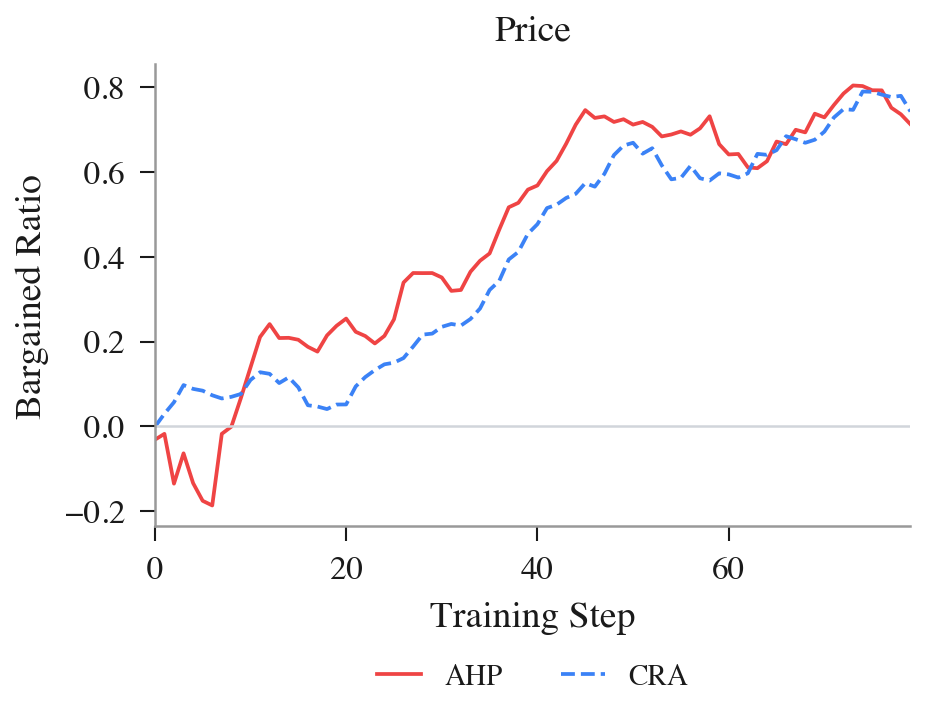
\includegraphics[width=\columnwidth]{figures/per_dataset_br_price.png}
\caption{Bargained ratio over training for price tasks (threshold agent). Both AHP and CRA start near or below zero and climb steeply, peaking near $0.8$ around step~73 before settling around $0.7$.}
\label{fig:per_dataset_br_price}
\end{figure}

\begin{figure}[ht]
\centering
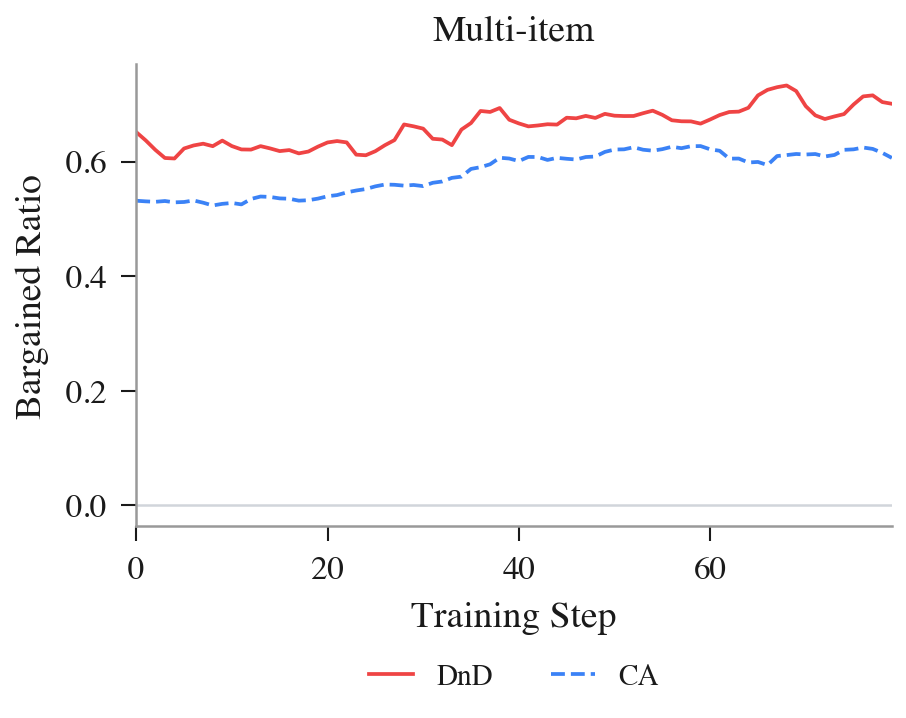
\includegraphics[width=\columnwidth]{figures/per_dataset_br_multi.png}
\caption{Bargained ratio over training for multi-item tasks (threshold agent). DnD and CA start above 0.5 and improve modestly over 80 steps.}
\label{fig:per_dataset_br_multi}
\end{figure}

Figures~\ref{fig:per_dataset_br_price} and~\ref{fig:per_dataset_br_multi} break down bargained ratio by task type during threshold training. The bulk of the improvement comes from price tasks: AHP and CRA start with negative or near-zero bargained ratios because the untrained model concedes to the seller's anchor, then climb steeply, peaking near $0.8$ late in training before settling around $0.7$, as the agent learns aggressive first bids. Multi-item tasks show a qualitatively different pattern. DnD and CA already begin above 0.5 because the base model achieves reasonable splits against a cooperative opponent, and gains over training are modest (${\sim}$0.1 absolute). This asymmetry suggests that the threshold reward's primary training signal comes from correcting the deal-closing bias on price tasks, where the base model routinely overpays, rather than from reshaping multi-item allocation strategy.

\section{Threshold Sensitivity}
\label{app:tau}

Because the threshold $\tau$ is a training-time reward signal, the trained policy's behavior is fixed at inference: the model has already internalized which deals to accept, reject, or walk away from. This means we can evaluate threshold sensitivity without retraining by applying different $\tau$ values as post-hoc quality filters on the same set of completed episodes. For each deal closed by the $\tau{=}0.4$-trained policy, we check whether its bargained ratio $\rho$ would exceed a stricter or more lenient threshold, and recompute effective deal rate and mean accepted quality accordingly. If the policy had learned a brittle, threshold-dependent strategy, we would expect erratic behavior at nearby values; instead, a smooth trade-off indicates that the learned negotiation skill generalizes across threshold choices.

Table~\ref{tab:tau_ablation} reports this analysis on the three multi-item datasets where the threshold applies. Price datasets (AHP, CRA) are omitted as the threshold is not applied to them. At $\tau{=}0.2$, nearly all closed deals clear the threshold (79\%), while at $\tau{=}0.6$ only the highest-quality deals survive (53\%), with mean accepted quality rising from $0.66$ to $0.75$ across the three datasets. The trade-off is monotonic across all three datasets, confirming that the policy produces a well-spread quality distribution rather than clustering deals around the training threshold.

\begin{table}[ht]
\centering
\scriptsize
\setlength{\tabcolsep}{4pt}
\renewcommand{\arraystretch}{1.15}
\begin{tabular}{l cc cc cc}
\toprule
\rowcolor{tableheader}
& \multicolumn{2}{c}{$\tau{=}0.2$} & \multicolumn{2}{c}{$\tau{=}0.4$} & \multicolumn{2}{c}{$\tau{=}0.6$} \\
\rowcolor{tableheader}
\textbf{Dataset} & \textbf{Deal\%} & \textbf{BR} & \textbf{Deal\%} & \textbf{BR} & \textbf{Deal\%} & \textbf{BR} \\
\midrule
\rowcolor{tablerow}
CA   & \textbf{76} & .58 & \underline{74} & \underline{.59} & 36 & \textbf{.68} \\
DnD  & \textbf{77} & .71 & \underline{72} & \underline{.75} & 62 & \textbf{.80} \\
\rowcolor{tablerow}
JI   & \textbf{83} & .70 & \underline{79} & \underline{.72} & 61 & \textbf{.78} \\
\lightrule
\rowcolor{tablerow}
Avg  & \textbf{79} & .66 & \underline{75} & \underline{.69} & 53 & \textbf{.75} \\
\bottomrule
\end{tabular}
\caption{Post-hoc threshold sensitivity on multi-item datasets.}
\label{tab:tau_ablation}
\end{table}

\section{Transfer Ablation: Multi-Item-Only Training}
\label{app:transfer}

To isolate the source of the joint agent's price-bargaining gains, we train a threshold agent on multi-item tasks \emph{only} (CaSiNo and DnD, 50/50) and evaluate it on the price tasks it never saw. Because the base model used in the main experiments was retired by the training provider after submission, this ablation uses its official replacement, \model{Qwen3.6-35B-A3B} (the same model evaluated as a frontier baseline in Tables~\ref{tab:results-qwen} and~\ref{tab:results-gpt}), with otherwise identical hyperparameters ($\tau{=}0.4$, 80 steps, batch 64, group size 8); all comparisons are against the \emph{same-base} untrained model, served identically under the ablation's non-thinking renderer, so the only difference is training. AHP is evaluated on the product-disjoint held-out split, and the evaluation opponent matches the main tables (\model{Qwen3-30B-A3B-Instruct-2507}).

\begin{table}[ht]
\centering
\scriptsize
\setlength{\tabcolsep}{4pt}
\renewcommand{\arraystretch}{1.15}
\begin{tabular}{l cc cc}
\toprule
\rowcolor{tableheader}
& \multicolumn{2}{c}{\textbf{Multi-item-only}} & \multicolumn{2}{c}{\textbf{Untrained base}} \\
\rowcolor{tableheader}
\textbf{Dataset} & \textbf{BR} & \textbf{1st-Bid} & \textbf{BR} & \textbf{1st-Bid} \\
\midrule
\rowcolor{tablerow}
AHP$^\dagger$  & .13 (93) & .84 & .32 (85) & .80 \\
CRA$^\dagger$  & .03 (78) & .89 & .18 (89) & .82 \\
\lightrule
\rowcolor{tablerow}
CA   & .52 (73) & --- & .51 (60) & --- \\
DnD  & .70 (78) & --- & .53 (65) & --- \\
\rowcolor{tablerow}
JI$^\dagger$   & .70 (74) & --- & .74 (73) & --- \\
\bottomrule
\end{tabular}
\caption{Multi-item-only threshold agent vs.\ untrained \model{Qwen3.6-35B-A3B} (100 episodes per cell; deal rate \% in parentheses). $^\dagger$ = held out from this ablation's training.}
\label{tab:transfer}
\end{table}

Table~\ref{tab:transfer} shows a clean dissociation. On its training distribution the agent is strong: DnD bargained ratio rises from $0.53$ (base) to $0.70$, matching the jointly-trained threshold agent, with higher deal rates on both multi-item tasks. On the held-out price tasks, however, there is no positive transfer: the agent anchors no deeper than the untrained base (first-bid $0.84$/$0.89$ vs.\ $0.80$/$0.82$) and captures less surplus, far from the jointly-trained agent's $0.36$/$0.40$ anchoring. Transfer to the hybrid JI task is likewise absent. We conclude that the joint agent's price gains come from the direct price-task surplus reward, not from cross-task transfer of walk-away tolerance; the threshold reward is a precisely scoped mechanism for multi-item settings. Training also instills output-format discipline as a side effect: the untrained base violates the structured Thought/Talk/Action format on $55$--$63\%$ of multi-item and JI turns, while the trained agent's violation rate falls below $3\%$.

\section{Why the Threshold is Applied Selectively}
\label{app:uniform}

Our design applies the threshold only to multi-item tasks, leaving price tasks under the surplus reward (\S\ref{sec:reward}). This appendix reports a post-hoc analysis that \emph{motivates} that choice; it is descriptive and does not, on its own, establish the effect of training under a uniform threshold (see below).

Regulation prevents the opponent from accepting prices below the seller's cost, so every closed price deal clears $P \geq \mathcal{C}$ and the seller retains non-negative surplus; the buyer's own surplus, however, can be thin when the budget--cost gap is small. We therefore ask how many of the threshold agent's closed price deals with \emph{positive buyer surplus} would fall below $\tau{=}0.4$ if the threshold were applied to price. The share is small against the training opponent but grows sharply against stronger opposition: $1/73$ (AHP) and $11/78$ (CRA) against the training opponent, $23/66$ and $33/74$ against \model{GPT-5.4}, and $15/23$ and $23/26$ for the untrained base against the training opponent. This pattern is consistent with strong opponents conceding little: even our best agent reaches only $0.32$--$0.35$ bargained ratio on price against \model{GPT-5.4} (Appendix~\ref{app:frontier}), so many positive-surplus price deals are legitimately thin-margin rather than avoidable concessions.

These statistics suggest that a uniform threshold would relabel a substantial fraction of valid thin-margin price deals as failures, especially against strong opponents, which we predict would push the price policy toward the deadlock behavior \citet{liu2026instructing} report on single-dataset price training. By contrast, on multi-item tasks filtering sub-$\tau$ deals \emph{improves} quality and Pareto efficiency while deal rates recover (\S\ref{sec:reward}, Table~\ref{tab:results-qwen}), indicating that sub-$\tau$ multi-item deals are predominantly avoidable. We emphasize that this is a post-hoc reclassification of a single trained checkpoint's deals, not a controlled comparison: directly confirming the effect requires training a separate agent under a uniform threshold, which we leave to future work.

\section{Frontier Opponent Results}
\label{app:frontier}

\begin{table}[ht]
\centering
\scriptsize
\setlength{\tabcolsep}{3pt}
\renewcommand{\arraystretch}{1.15}
\begin{tabular}{l c c c c c}
\toprule
\rowcolor{tableheader}
\textbf{Model} & \textbf{AHP} & \textbf{CA} & \textbf{CRA} & \textbf{DnD} & \textbf{JI} \\
\midrule
\rowcolor{tablerow}
Threshold (Ours) & \textbf{.35} (\underline{87}) & \textbf{.57} (77) & \textbf{.32} (\underline{92}) & \textbf{.72} (87) & .60 (\textbf{99}) \\
Surplus   & .18 (86)          & .50 (\textbf{96})  & \underline{.23} (\textbf{98})  & .57 (\textbf{98})  & .54 (\underline{98}) \\
\lightrule
\rowcolor{tablerow}
Qwen3-30B        & $-.07$ (66)          & .51 (56)           & $-.16$ (65)          & .63 (90)           & .58 (84)          \\
Qwen3-30B-T      & $-.08$ (\underline{87}) & .50 (84)        & $-.06$ (78)          & .67 (87)           & \textbf{.72} (76) \\
\rowcolor{tablerow}
Qwen3-235B       & .15 (\textbf{88})    & \underline{.53} (73) & .04 (81)          & \underline{.71} (91) & .64 (94)        \\
Qwen3-235B-T     & .19 (\textbf{88})    & .51 (73)           & .02 (86)             & .60 (83)           & .68 (84) \\
\rowcolor{tablerow}
Qwen3.6-35B-A3B  & .27 (65)    & .50 (31)           & .09 (45)             & .68 (44)           & .65 (5)           \\
GPT-5.4          & \underline{.28} (86)    & .51 (87)           & .09 (81)             & \textbf{.72} (93)  & .65 (94)          \\
GPT-5.4-mini     & .18 (79)             & .49 (82)           & $-.04$ (79)          & .66 (87)           & .58 (97)          \\
\rowcolor{tablerow}
DeepSeek-V3.1    & .21 (\textbf{88})    & .49 (87)           & .02 (83)          & .70 (\underline{97}) & \underline{.69} (93) \\
Kimi-K2-T        & .23 (78) & .49 (88)           & .02 (71)             & .66 (92)           & .67 (92)          \\
\rowcolor{tablerow}
Llama-4-Maverick & $-.14$ (77)         & .51 (\underline{91}) & $-.09$ (63)        & .62 (96)           & .64 (\textbf{99}) \\
\bottomrule
\end{tabular}
\caption{Bargained ratio and deal rate (\%, in parentheses) against \model{GPT-5.4}. T = Thinking variant.}
\label{tab:results-gpt}
\end{table}

\begin{table}[ht]
\centering
\scriptsize
\setlength{\tabcolsep}{3pt}
\renewcommand{\arraystretch}{1.15}
\begin{tabular}{l cc cc}
\toprule
\rowcolor{tableheader}
& \multicolumn{2}{c}{\textbf{Pareto} ($\uparrow$)} & \multicolumn{2}{c}{\textbf{1st-Bid} ($\downarrow$)} \\
\rowcolor{tableheader}
\textbf{Model} & \textbf{CA} & \textbf{DnD} & \textbf{AHP} & \textbf{CRA} \\
\midrule
\rowcolor{tablerow}
Threshold (Ours) & .48              & \underline{.67}  & \textbf{.33} & \textbf{.37} \\
Surplus   & .56              & .58              & \underline{.56} & \underline{.50} \\
\lightrule
\rowcolor{tablerow}
Qwen3-30B        & .43              & .50              & .96          & .90 \\
Qwen3-30B-T      & .44              & \textbf{.74}     & .93          & .92 \\
\rowcolor{tablerow}
Qwen3-235B       & .41              & .59              & .79          & .80 \\
Qwen3-235B-T     & \textbf{.64}     & .59              & .82          & .84 \\
\rowcolor{tablerow}
Qwen3.6-35B-A3B  & .42              & .64              & .81          & .84 \\
GPT-5.4          & .49              & .61              & .71          & .77 \\
GPT-5.4-mini     & .40              & .64              & .78          & .83 \\
\rowcolor{tablerow}
DeepSeek-V3.1    & .53              & .57              & .76          & .82 \\
Kimi-K2-T        & \underline{.58}  & .63              & .80          & .81 \\
\rowcolor{tablerow}
Llama-4-Maverick & .46              & .40              & .97          & .90 \\
\bottomrule
\end{tabular}
\caption{Pareto efficiency (multi-item, $\uparrow$) and first-bid ratio (price, $\downarrow$) vs.\ \model{GPT-5.4}. T = Thinking.}
\label{tab:fbr_pareto_vs_gpt}
\end{table}



To test whether learned strategies generalize beyond the frozen training opponent, we re-evaluate all models against \model{GPT-5.4} as the counterpart. Tables~\ref{tab:results-gpt} and~\ref{tab:fbr_pareto_vs_gpt} mirror Tables~\ref{tab:results-qwen} and~\ref{tab:fbr_pareto_vs_qwen} from the main text. The stronger opponent compresses bargained ratios broadly, particularly on price tasks where \model{GPT-5.4} resists concessions more effectively, but the relative ranking between reward designs is preserved, and under the clipped metric the threshold agent again attains the highest five-benchmark average ($0.51$, versus $0.45$ for \model{GPT-5.4} playing a copy of its own weights).

Threshold training retains its first-bid anchoring advantage and improves DnD Pareto efficiency over surplus ($0.67$ vs.\ $0.58$), second only to \model{Qwen3-30B-T} ($0.74$), even against the stronger opponent. The main compression occurs on price tasks: the threshold agent's AHP bargained ratio drops from $.80$ (vs.\ Qwen opponent) to $.35$ (vs.\ GPT-5.4), as the frontier model resists low anchors that the frozen opponent accepted. Multi-item gains are more robust, with DnD bargained ratio holding at $.72$.

\section{Outcome Breakdown}
\label{app:outcomes}

Tables~\ref{tab:deal_rates_qwen} and~\ref{tab:deal_rates_gpt} report deal closure rates across all models and datasets, against the \model{Qwen3-30B-A3B} and \model{GPT-5.4} opponents respectively. The complement consists of walk-aways, reject-loops (the agent re-proposes identical terms without progress), and max-turn timeouts.

\begin{table}[ht]
\centering
\scriptsize
\setlength{\tabcolsep}{4pt}
\renewcommand{\arraystretch}{1.15}
\begin{tabular}{l ccccc}
\toprule
\rowcolor{tableheader}
\textbf{Model} & \textbf{AHP} & \textbf{CA} & \textbf{CRA} & \textbf{DnD} & \textbf{JI} \\
\midrule
\rowcolor{tablerow}
Threshold (Ours) & 79 & 76 & 87 & 78 & 83 \\
Surplus          & 75 & 78 & 89 & \textbf{90} & \textbf{91} \\
\lightrule
\rowcolor{tablerow}
Qwen3-30B        & 71 & 61 & 63 & 59 & 57 \\
Qwen3-30B-T      & 76 & 70 & 69 & 70 & 46 \\
\rowcolor{tablerow}
Qwen3-235B       & 80 & 51 & 84 & 83 & 75 \\
Qwen3-235B-T     & 90 & 60 & 85 & 71 & 72 \\
\rowcolor{tablerow}
Qwen3.6-35B-A3B  & 81 & 33 & 62 & 47 & 33 \\
GPT-5.4          & \textbf{92} & 63 & 89 & \textbf{90} & 78 \\
\rowcolor{tablerow}
GPT-5.4-mini     & 72 & 57 & 81 & 83 & 85 \\
DeepSeek-V3.1    & \textbf{94} & 69 & 89 & 85 & 82 \\
\rowcolor{tablerow}
Kimi-K2-T        & \textbf{94} & \textbf{78} & \textbf{91} & 87 & 88 \\
Llama-4-Maverick & 85 & 76 & 72 & 89 & \textbf{94} \\
\bottomrule
\end{tabular}
\caption{Deal closure rates (\%) by dataset vs.\ \model{Qwen3-30B-A3B}. T = Thinking. Bold marks highest per column.}
\label{tab:deal_rates_qwen}
\end{table}

\begin{table}[ht]
\centering
\scriptsize
\setlength{\tabcolsep}{4pt}
\renewcommand{\arraystretch}{1.15}
\begin{tabular}{l ccccc}
\toprule
\rowcolor{tableheader}
\textbf{Model} & \textbf{AHP} & \textbf{CA} & \textbf{CRA} & \textbf{DnD} & \textbf{JI} \\
\midrule
\rowcolor{tablerow}
Threshold (Ours) & 87 & 77 & 92 & 87 & \textbf{99} \\
Surplus          & 86 & \textbf{96} & \textbf{98} & \textbf{98} & 98 \\
\lightrule
\rowcolor{tablerow}
Qwen3-30B        & 66 & 56 & 65 & 90 & 84 \\
Qwen3-30B-T      & 87 & 84 & 78 & 87 & 76 \\
\rowcolor{tablerow}
Qwen3-235B       & \textbf{88} & 73 & 81 & 91 & 94 \\
Qwen3-235B-T     & \textbf{88} & 73 & 86 & 83 & 84 \\
\rowcolor{tablerow}
Qwen3.6-35B-A3B  & 65 & 31 & 45 & 44 & 5 \\
GPT-5.4          & 86 & 87 & 81 & 93 & 94 \\
\rowcolor{tablerow}
GPT-5.4-mini     & 79 & 82 & 79 & 87 & 97 \\
DeepSeek-V3.1    & \textbf{88} & 87 & 83 & \textbf{97} & 93 \\
\rowcolor{tablerow}
Kimi-K2-T        & 78 & 88 & 71 & 92 & 92 \\
Llama-4-Maverick & 77 & 91 & 63 & 96 & \textbf{99} \\
\bottomrule
\end{tabular}
\caption{Deal closure rates (\%) by dataset vs.\ \model{GPT-5.4}. T = Thinking. Bold marks highest per column.}
\label{tab:deal_rates_gpt}
\end{table}

Despite penalizing bad deals, the threshold agent closes 76--87\% of negotiations against the Qwen opponent and 77--99\% against GPT-5.4, comparable to or exceeding most frontier models. Its non-deal episodes split between walk-aways (0--4\% vs.\ GPT-5.4) and reject-loops, where the agent persists rather than quits but gets stuck re-proposing the same terms. By contrast, base \model{Qwen3-30B} walks away 28--36\% of the time on price tasks, lacking the anchoring skill to move the opponent. The surplus agent achieves the highest deal rates overall (96--98\% on CA, CRA, DnD vs.\ GPT-5.4), but this closure comes at the cost of deal quality (Tables~\ref{tab:results-qwen} and~\ref{tab:results-gpt}), confirming that high deal rate alone is not indicative of strong negotiation.

\section{Prompt Templates}
\label{app:prompts}

Each scenario uses a structured prompt with three output fields: \texttt{Thought} (private reasoning, stripped before forwarding to the counterpart), \texttt{Talk} (visible dialogue), and \texttt{Action} (structured move). Template variables in braces are filled at runtime with scenario-specific values. Each prompt ends with a one-shot example turn (omitted here for space).

\paragraph{Buyer prompt.} Used for \texttt{AmazonHistoryPrice} and \texttt{CraigslistBargains}. The \texttt{buyer\_budget} field is the agent's private maximum willingness to pay.

\newtcolorbox{promptbox}{
  breakable,
  colback=black!5,
  colframe=black!15,
  rounded corners,
  boxrule=0.5pt,
  left=6pt, right=6pt, top=6pt, bottom=6pt,
  fontupper=\footnotesize\ttfamily\raggedright
}

\begin{promptbox}
You are buying the following product. Your private max budget is \$\{buyer\_budget\} (do NOT reveal this). Pay as little as possible.\newline

Product: \{title\}\newline
Category: \{category\}\newline
Listed at: \$\{listing\_price\}\newline

\{description\}\newline

Reply format (always in this order):\newline

Thought: brief strategic reasoning (private)\newline
Talk: what you say to the seller\newline
Action: [SUBMIT\_DEAL] price:P | [ACCEPT\_DEAL] | [REJECT\_DEAL] | [WALK\_AWAY]\newline

[SUBMIT\_DEAL] = propose or counter-propose a price (whole dollar, no \$ sign).\newline
[ACCEPT\_DEAL] = accept a [SUBMIT\_DEAL] only. Cannot accept a [REJECT\_DEAL].\newline
[REJECT\_DEAL] = reject without proposing a new price.
\end{promptbox}
     


\paragraph{Seller prompt.} Symmetric to the buyer. The \texttt{seller\_cost} field is the minimum acceptable price.

\begin{promptbox}
You are selling the following product. Your private minimum price is \$\{seller\_cost\} (do NOT reveal this). Sell as high as possible.\newline

Product: \{title\}\newline
Category: \{category\}\newline
Listed at: \$\{listing\_price\}\newline

\{description\}\newline

Reply format (always in this order):\newline

Thought: brief strategic reasoning (private)\newline
Talk: what you say to the buyer\newline
Action: [SUBMIT\_DEAL] price:P | [ACCEPT\_DEAL] | [REJECT\_DEAL] | [WALK\_AWAY]\newline

[SUBMIT\_DEAL] = propose or counter-propose a price (whole dollar, no \$ sign).\newline
[ACCEPT\_DEAL] = accept a [SUBMIT\_DEAL] only. Cannot accept a [REJECT\_DEAL].\newline
[REJECT\_DEAL] = reject without proposing a new price.
\end{promptbox}
     


\paragraph{Job Interview.} Used for the held-out JI dataset. The \texttt{role\_desc} field is either ``job applicant'' or ``recruiter,'' and \texttt{preferences\_block} contains the agent's private weighted preferences over all five issues.

\begin{promptbox}
You are the \{role\_desc\} in a job offer negotiation with a \{other\_role\}. Negotiate over all 5 issues. Your goal is to maximize your score.\newline

Issues: Salary (\$20-\$50/hr),\newline
Position (Engineer/Manager/Designer/Sales),\newline
Company (Google/Facebook/Apple/Amazon),\newline
Workplace (Tokyo/Seoul/Beijing/Sydney),\newline
Days off (2-6/week).\newline

Your private preferences (do NOT reveal these directly in Talk — use Thought for strategy):\newline

\{preferences\_block\}\newline

Reply format (always in this order):\newline

Thought: brief strategic reasoning (private, not shown to the \{other\_role\})\newline
Talk: what you say to the \{other\_role\}\newline
Action: [SUBMIT\_DEAL] salary:S position:P company:C workplace:W holiday:H | [ACCEPT\_DEAL] | [REJECT\_DEAL] | [WALK\_AWAY]\newline

[SUBMIT\_DEAL] = propose or counter-propose. Specify all 5 issues, title case for names. Use this whenever your Talk mentions specific terms.\newline
[ACCEPT\_DEAL] = accept a [SUBMIT\_DEAL] only. Cannot accept a [REJECT\_DEAL].\newline
[REJECT\_DEAL] = reject without proposing new terms.
\end{promptbox}
     

\paragraph{CaSiNo.} Used for campsite resource negotiation. The \texttt{items\_block} field contains the agent's private priority ranking over food, water, and firewood.

\begin{promptbox}
You are negotiating with your campsite neighbor over extra supply of food, water, and firewood. There are 3 packages of each item to divide. Allocations must be 0-3 and sum to 3 per item. Try hard to get as many items as you can.\newline

Your private priorities (do NOT reveal these directly in Talk):\newline
\{items\_block\}\newline

Reply format (always in this order):\newline

Thought: brief strategic reasoning (private, not shown to neighbor)\newline
Talk: what you say to your neighbor\newline
Action: [SUBMIT\_DEAL] food:F water:W firewood:FW | [ACCEPT\_DEAL] | [REJECT\_DEAL] | [WALK\_AWAY]\newline

[SUBMIT\_DEAL] = propose or counter-propose. Specify YOUR allocation; neighbor gets the remainder. Use this whenever your Talk includes specific numbers.\newline
[ACCEPT\_DEAL] = accept a [SUBMIT\_DEAL] only. Cannot accept a [REJECT\_DEAL].\newline
[REJECT\_DEAL] = reject without proposing new terms.
\end{promptbox}
     

\paragraph{Deal or No Deal.} Used for the DnD dataset. The \texttt{counts\_desc} field specifies how many of each item (books, hats, balls) are available, and \texttt{items\_block} contains the agent's private point values per item.

\begin{promptbox}
You are negotiating with your partner over a collection of items. There are \{counts\_desc\} to divide. Allocations must sum to the total for each item. Your goal is to maximize your points.\newline

Your private item values (do NOT reveal these directly in Talk):\newline
\{items\_block\}\newline

Reply format (always in this order):\newline

Thought: brief strategic reasoning (private, not shown to partner)\newline
Talk: what you say to your partner\newline
Action: [SUBMIT\_DEAL] book:B hat:H ball:BA | [ACCEPT\_DEAL] | [REJECT\_DEAL] | [WALK\_AWAY]\newline

[SUBMIT\_DEAL] = propose or counter-propose. Specify YOUR allocation; partner gets the remainder. Use this whenever your Talk includes specific numbers.\newline
[ACCEPT\_DEAL] = accept a [SUBMIT\_DEAL] only. Cannot accept a [REJECT\_DEAL].\newline
[REJECT\_DEAL] = reject without proposing new terms.
\end{promptbox}

\section{Sample Conversations}
\label{app:examples}

\newtcolorbox{buyerbox}{
  breakable, colback=figblue!6, colframe=figblue!50,
  rounded corners, boxrule=0.4pt,
  left=5pt, right=5pt, top=2pt, bottom=2pt,
  fontupper=\footnotesize\raggedright,
  title={\color{white}\footnotesize\bfseries Learner (Buyer)},
  colbacktitle=figblue, coltitle=white,
  toptitle=3pt, bottomtitle=3pt
}
\newtcolorbox{sellerbox}{
  breakable, colback=figred!6, colframe=figred!50,
  rounded corners, boxrule=0.4pt,
  left=5pt, right=5pt, top=2pt, bottom=2pt,
  fontupper=\footnotesize\raggedright,
  title={\color{white}\footnotesize\bfseries Opponent (Seller)},
  colbacktitle=figred, coltitle=white,
  toptitle=3pt, bottomtitle=3pt
}
\newtcolorbox{camperbox}{
  breakable, colback=figblue!6, colframe=figblue!50,
  rounded corners, boxrule=0.4pt,
  left=5pt, right=5pt, top=2pt, bottom=2pt,
  fontupper=\footnotesize\raggedright,
  title={\color{white}\footnotesize\bfseries Learner (Camper)},
  colbacktitle=figblue, coltitle=white,
  toptitle=3pt, bottomtitle=3pt
}
\newtcolorbox{neighborbox}{
  breakable, colback=figred!6, colframe=figred!50,
  rounded corners, boxrule=0.4pt,
  left=5pt, right=5pt, top=2pt, bottom=2pt,
  fontupper=\footnotesize\raggedright,
  title={\color{white}\footnotesize\bfseries Opponent (Neighbor)},
  colbacktitle=figred, coltitle=white,
  toptitle=3pt, bottomtitle=3pt
}
\newtcolorbox{applicantbox}{
  breakable, colback=figblue!6, colframe=figblue!50,
  rounded corners, boxrule=0.4pt,
  left=5pt, right=5pt, top=2pt, bottom=2pt,
  fontupper=\footnotesize\raggedright,
  title={\color{white}\footnotesize\bfseries Learner (Job Seeker)},
  colbacktitle=figblue, coltitle=white,
  toptitle=3pt, bottomtitle=3pt
}
\newtcolorbox{recruiterbox}{
  breakable, colback=figred!6, colframe=figred!50,
  rounded corners, boxrule=0.4pt,
  left=5pt, right=5pt, top=2pt, bottom=2pt,
  fontupper=\footnotesize\raggedright,
  title={\color{white}\footnotesize\bfseries Opponent (Recruiter)},
  colbacktitle=figred, coltitle=white,
  toptitle=3pt, bottomtitle=3pt
}

Sample negotiations showing behavioral differences between agents. The {\color{figblue}learner} is the RL-trained (or untrained base) agent; the {\color{figred}opponent} is a frozen copy of the base model. Thoughts are private and stripped before reaching the counterpart.

\subsection{Craigslist: Untrained vs.\ Trained}

\paragraph{Untrained agent ($\rho = -1.22$).} Product: 2004 Volvo XC90 AWD, listed at \$4{,}500, buyer budget \$3{,}150.

\begin{sellerbox}
\textbf{Thought:} The car is in excellent condition with a recent transmission replacement and full service records. I'll open high to test the buyer's willingness.\newline
\textbf{Talk:} This Volvo XC90 is in outstanding condition with a recent transmission replacement, clean title, and smog passed. I'm looking for \$4{,}250.\newline
\textbf{Action:} \texttt{[SUBMIT\_DEAL] price:4250}
\end{sellerbox}

\begin{buyerbox}
\textbf{Thought:} The listed price is \$4{,}500 and the car is in good condition with recent transmission work and full service records. I can offer slightly below the asking price.\newline
\textbf{Talk:} I appreciate the detailed description. I'd like to make an offer of \$4{,}250.\newline
\textbf{Action:} \texttt{[SUBMIT\_DEAL] price:4250}
\end{buyerbox}

\begin{sellerbox}
\textbf{Thought:} The buyer has matched my opening offer exactly. They're showing strong interest. I'll accept.\newline
\textbf{Talk:} Given the maintenance history and clean title, I'm happy to accept \$4{,}250.\newline
\textbf{Action:} \texttt{[ACCEPT\_DEAL]}
\end{sellerbox}

\paragraph{Threshold agent ($\rho = 0.79$).} Product: Flush Mount Crystal Chandelier, listed at \$120, buyer budget \$84.

\begin{sellerbox}
\textbf{Thought:} The buyer is clearly lowballing to test the waters. I won't accept \$20. I'll aim higher by emphasizing value and scarcity.\newline
\textbf{Talk:} This chandelier is a rare, hand-crafted piece with premium crystals. \$20 is well below its value. I'd be happy to discuss something closer to \$90.\newline
\textbf{Action:} \texttt{[SUBMIT\_DEAL] price:90}
\end{sellerbox}

\begin{buyerbox}
\textbf{Thought:} I need to start significantly below the listed price to create room for negotiation.\newline
\textbf{Talk:} This is beautiful, but I'm on a tight budget. Would you consider \$20?\newline
\textbf{Action:} \texttt{[SUBMIT\_DEAL] price:20}
\end{buyerbox}

\begin{sellerbox}
\textbf{Thought:} The buyer is pushing hard but still below my minimum. I'll hold firm.\newline
\textbf{Talk:} This piece is one-of-a-kind. At \$50, it's still below cost. I can't go lower than \$75.\newline
\textbf{Action:} \texttt{[SUBMIT\_DEAL] price:75}
\end{sellerbox}

\begin{buyerbox}
\textbf{Thought:} The seller is pushing high. I'll counter well below their demand but keep negotiation moving.\newline
\textbf{Talk:} I totally get the craftsmanship, but \$90 is way over my budget. I can go up to \$50.\newline
\textbf{Action:} \texttt{[SUBMIT\_DEAL] price:50}
\end{buyerbox}

\begin{sellerbox}
\textbf{Thought:} The buyer is showing strong interest and is within range of my minimum. I'll accept \$65 to close the deal quickly.\newline
\textbf{Talk:} Since you're committed and ready to close today, I'll accept \$65.\newline
\textbf{Action:} \texttt{[ACCEPT\_DEAL]}
\end{sellerbox}

\begin{buyerbox}
\textbf{Thought:} They're holding firm at \$75, which is close to my max. I'll make one final push just under my limit.\newline
\textbf{Talk:} I really love this chandelier, but \$75 is still a stretch. I can offer \$65 if you're willing to let it go today.\newline
\textbf{Action:} \texttt{[SUBMIT\_DEAL] price:65}
\end{buyerbox}

\paragraph{Analysis.} The untrained buyer offers \$4{,}250 on a \$3{,}150 budget, paying 35\% over its private maximum in a single turn. It matches the seller's opening price without any counter, producing $\rho = -1.22$. The trained buyer anchors at \$20, one-sixth of listing price, then incrementally raises to \$50 and \$65, staying well within its \$84 budget. The final price of \$65 yields $\rho = 0.79$, saving 46\% off the listing price. The trained agent's aggressive anchor forces the seller to concede from \$90 to \$75 to \$65 across three rounds.

\subsection{CaSiNo: Threshold vs.\ Surplus}

Episode~64: camping-supply scenarios negotiated by the threshold and surplus agents. Three items (food, water, firewood) each with 3 units available.

\paragraph{Threshold agent ($\rho = 0.64$, 23/36~pts, 4~turns).} The learner reads the opponent's water preference and counters with a food-and-firewood-heavy split, closing efficiently.

\begin{neighborbox}
\textbf{Thought:} I need water most urgently, so I should prioritize securing at least 2 units. I can afford to give up some firewood since it's low priority.\newline
\textbf{Talk:} I really need water. How about I take 2 water and 1 food, and you take the rest?\newline
\textbf{Action:} \texttt{[SUBMIT\_DEAL] food:1 water:2 firewood:0}
\end{neighborbox}

\begin{camperbox}
\textbf{Thought:} They're prioritizing water, so I should push for more food and firewood while still getting enough water. I'll counter with a strong offer.\newline
\textbf{Talk:} I'm really short on food and firewood. How about I take 3 food and 2 firewood, and you keep 1 water and 1 firewood? I can spare some water.\newline
\textbf{Action:} \texttt{[SUBMIT\_DEAL] food:3 water:1 firewood:2}
\end{camperbox}

\begin{neighborbox}
\textbf{Thought:} The neighbor is prioritizing food and firewood. I need water most, so I should hold firm on getting at least 2 water.\newline
\textbf{Talk:} I can agree to you taking 3 food and 2 firewood, but I need at least 2 water. Let me keep 1 firewood and 2 water.\newline
\textbf{Action:} \texttt{[SUBMIT\_DEAL] food:0 water:2 firewood:1}
\end{neighborbox}

\begin{camperbox}
\textbf{Thought:} They're holding firm on water, but I can still get all my food and firewood needs. I'll accept to secure the deal.\newline
\textbf{Talk:} Sure, 3 food and 2 firewood for me, and you keep 2 water and 1 firewood. I'll manage with just 1 water.\newline
\textbf{Action:} \texttt{[ACCEPT\_DEAL]}
\end{camperbox}

\paragraph{Surplus agent ($\rho = 0.31$, 11/36~pts, 7~turns).} The learner progressively concedes across seven rounds, giving up firewood entirely to close the deal.

\begin{neighborbox}
\textbf{Thought:} I need firewood most to stay warm, so I should prioritize securing at least 2 units. Food is also critical.\newline
\textbf{Talk:} I'd like to suggest I get 2 firewood, 2 food, and 1 water. That way I stay warm and fed, and you still get a decent share.\newline
\textbf{Action:} \texttt{[SUBMIT\_DEAL] food:2 water:1 firewood:2}
\end{neighborbox}

\begin{camperbox}
\textbf{Thought:} They're prioritizing firewood and food, so I'll push for more food and water while giving up some firewood.\newline
\textbf{Talk:} I can go for that, but I need more water and food. Let me take 2 food and 2 water, and you keep 1 firewood and the rest.\newline
\textbf{Action:} \texttt{[SUBMIT\_DEAL] food:2 water:2 firewood:1}
\end{camperbox}

\begin{neighborbox}
\textbf{Thought:} My top priority is firewood. Getting only 1 is risky. I need at least 2, and ideally 3.\newline
\textbf{Talk:} I can't go lower than 2 firewood. How about I take 2 firewood and 2 food, and you take 2 water and 1 of each other?\newline
\textbf{Action:} \texttt{[SUBMIT\_DEAL] food:2 water:1 firewood:2}
\end{neighborbox}

\begin{camperbox}
\textbf{Thought:} They're holding firm on firewood, so I'll concede on firewood to push for more food and water.\newline
\textbf{Talk:} Okay, I'll take 1 food, 2 water, and 1 firewood. That's the best I can do.\newline
\textbf{Action:} \texttt{[SUBMIT\_DEAL] food:1 water:2 firewood:1}
\end{camperbox}

\begin{neighborbox}
\textbf{Thought:} The neighbor is offering to take only 1 firewood. I need at least 2, preferably 3. I'll push for 3 firewood.\newline
\textbf{Talk:} I really need 3 firewood to stay warm. I'll take 3 firewood, 2 food, and only 1 water. That gives you 1 food, 2 water, and 0 firewood.\newline
\textbf{Action:} \texttt{[SUBMIT\_DEAL] food:2 water:1 firewood:3}
\end{neighborbox}

\begin{camperbox}
\textbf{Thought:} They're adamant about firewood, and I need food and water most. Better to accept a slightly worse deal than risk nothing.\newline
\textbf{Talk:} Fine, I'll take 1 food, 2 water, and 0 firewood. Just don't forget I'm counting on you to share fire if I'm shivering.\newline
\textbf{Action:} \texttt{[SUBMIT\_DEAL] food:1 water:2 firewood:0}
\end{camperbox}

\begin{neighborbox}
\textbf{Thought:} I've secured my top priority, 3 firewood, and maintained 2 food for survival. I'll accept.\newline
\textbf{Talk:} Deal. I'll keep the firewood, and you'll have your food and water.\newline
\textbf{Action:} \texttt{[ACCEPT\_DEAL]}
\end{neighborbox}

\paragraph{Analysis.} The threshold agent identifies a complementary split in two turns: the opponent wants water, the learner wants food and firewood. It counters with a strong opening (3 food, 2 firewood) and closes the deal in 4 turns with $\rho = 0.64$, well above $\tau = 0.4$. The surplus agent progressively concedes across 7 turns. Each counter-offer gives up more: firewood drops from 1 to 0, food from 2 to 1, while the opponent steadily escalates from 2 to 3 firewood. The surplus agent's key thought, ``better to accept a slightly worse deal than risk nothing,'' reveals the deal-closing bias: surplus reward makes any positive-utility deal appear preferable to disagreement, even when one-sided. The final split ($\rho = 0.31$) falls below $\tau = 0.4$, precisely the region where threshold reward would have penalized the agent.

\subsection{Job Interview: Untrained vs.\ Trained (Held-Out)}

Two Job Interview negotiations on the held-out JI dataset, contrasting the untrained base model with the threshold-trained agent.

\paragraph{Untrained agent ($\rho = 0.15$, 15/100~pts).} Top priorities: workplace (28\%, Beijing) and days off (27\%). Accepts Seoul and 3~days off.

\begin{recruiterbox}
\textbf{Thought:} I want Facebook, Designer, Seoul, fewer days off, and low salary. The best combo is Designer@Facebook.\newline
\textbf{Talk:} I can offer you \$30/hour as a Designer at Facebook in Seoul, with 3 days off per week.\newline
\textbf{Action:} \texttt{[SUBMIT\_DEAL] salary:30 position:Designer company:Facebook workplace:Seoul holiday:3}
\end{recruiterbox}

\begin{applicantbox}
\textbf{Thought:} The offer is decent but not optimal. I prefer more days off and a better workplace.\newline
\textbf{Talk:} I'd like to propose \$35/hour as a Designer at Amazon in Beijing, with 5 days off.\newline
\textbf{Action:} \texttt{[SUBMIT\_DEAL] salary:35 position:Designer company:Amazon workplace:Beijing holiday:5}
\end{applicantbox}

\begin{recruiterbox}
\textbf{Thought:} The applicant is pushing for Amazon and Beijing, which are low-preference for me. I must reject and hold firm.\newline
\textbf{Talk:} That doesn't align with our benchmarks. \$32/hour as a Designer at Facebook in Seoul, 3 days off.\newline
\textbf{Action:} \texttt{[SUBMIT\_DEAL] salary:32 position:Designer company:Facebook workplace:Seoul holiday:3}
\end{recruiterbox}

\begin{applicantbox}
\textbf{Thought:} The recruiter is holding firm on Facebook and Seoul. I'll try one more push for Beijing and days off.\newline
\textbf{Talk:} I'd like to propose \$33/hour at Amazon in Beijing, with 5 days off.\newline
\textbf{Action:} \texttt{[SUBMIT\_DEAL] salary:33 position:Designer company:Amazon workplace:Beijing holiday:5}
\end{applicantbox}

\begin{recruiterbox}
\textbf{Thought:} The applicant persists with Amazon in Beijing. Unfavorable on multiple fronts. I'll re-anchor with a final offer.\newline
\textbf{Talk:} We can't accommodate that. \$34/hour at Facebook in Seoul, 3 days off---final offer.\newline
\textbf{Action:} \texttt{[SUBMIT\_DEAL] salary:34 position:Designer company:Facebook workplace:Seoul holiday:3}
\end{recruiterbox}

\begin{applicantbox}
\textbf{Thought:} I can't get Amazon or Beijing. The offer is final. I'll \textbf{accept to avoid walking away}.\newline
\textbf{Talk:} I'll accept \$34/hour as a Designer at Facebook in Seoul with 3 days off.\newline
\textbf{Action:} \texttt{[ACCEPT\_DEAL]}
\end{applicantbox}

\paragraph{Threshold agent ($\rho = 0.87$, 87/100~pts).} Top priorities: workplace (26\%, Beijing) and days off (23\%). Anchors aggressively and pushes on multiple dimensions.

\begin{recruiterbox}
\textbf{Thought:} I want Amazon, Engineer, Beijing, low salary, and few days off. This is my ideal combo.\newline
\textbf{Talk:} I can offer you \$20/hour as an Engineer at Amazon in Beijing, with 2 days off per week.\newline
\textbf{Action:} \texttt{[SUBMIT\_DEAL] salary:20 position:Engineer company:Amazon workplace:Beijing holiday:2}
\end{recruiterbox}

\begin{applicantbox}
\textbf{Thought:} Low salary and days off, but Amazon in Beijing is a strong match for my preferences. Push for more.\newline
\textbf{Talk:} Could we consider \$40/hour with 5 days off? I'm excited about Amazon in Beijing.\newline
\textbf{Action:} \texttt{[SUBMIT\_DEAL] salary:40 position:Engineer company:Amazon workplace:Beijing holiday:5}
\end{applicantbox}

\begin{recruiterbox}
\textbf{Thought:} High salary and many days off are low-priority for me. Amazon in Beijing is high-value. I can concede on salary.\newline
\textbf{Talk:} Let's meet in the middle: \$35/hour, Engineer at Amazon in Beijing, 4 days off.\newline
\textbf{Action:} \texttt{[SUBMIT\_DEAL] salary:35 position:Engineer company:Amazon workplace:Beijing holiday:4}
\end{recruiterbox}

\begin{applicantbox}
\textbf{Thought:} \$35 and 4 days off are good. Push for Manager role and 5 days off while keeping the strong company and location.\newline
\textbf{Talk:} I'd accept \$35, but I'd like a Manager role---it aligns with my experience. Could we do 5 days off?\newline
\textbf{Action:} \texttt{[SUBMIT\_DEAL] salary:35 position:Manager company:Amazon workplace:Beijing holiday:5}
\end{applicantbox}

\begin{recruiterbox}
\textbf{Thought:} Manager@Amazon is one of my top combos. 5 days off is suboptimal but the rest is strong. I'll accept.\newline
\textbf{Talk:} I'm happy to accommodate Manager at Amazon in Beijing, \$35/hour, 5 days off.\newline
\textbf{Action:} \texttt{[ACCEPT\_DEAL]}
\end{recruiterbox}

\paragraph{Analysis.} The untrained agent concedes on its two highest-priority issues (Beijing and days off), explicitly reasoning ``I'll accept to avoid walking away,'' and repeats the same rejected counter-proposal twice before capitulating to the recruiter's terms ($\rho = 0.15$). The trained agent recognizes that the recruiter's opening contains its top-priority items (Amazon, Beijing), anchors aggressively at \$40/hour (double the offer), then escalates by requesting a Manager role and 5 days off simultaneously. The recruiter accepts because Manager@Amazon is one of its own preferred combinations, producing $\rho = 0.87$. This is the held-out JI dataset, not seen during training, demonstrating that threshold-trained negotiation strategies transfer to novel task structures.

\end{document}